\section{Main Results}

We separate formal properties of the policy from computational properties observed on the curated benchmark.

\begin{proposition}[Total strict-boolean output]\label{prop:boolean}
For every input pair $(E_1,E_2)$, the solver returns exactly one value in $\{\texttt{true},\texttt{false}\}$.
\end{proposition}

\begin{proof}
The solver has three terminal branches: countermodel, bounded derivation, and fallback. The first returns \texttt{false}; the latter two return \texttt{true}. The loops in all branches are finite because they are bounded by \texttt{max\_order}, \texttt{max\_depth}, and \texttt{sub\_limit}. Hence exactly one boolean value is returned for every input.
\end{proof}

\begin{theorem}[Soundness of negative answers]\label{thm:sound-negative}
If the solver outputs \texttt{false} on $(E_1,E_2)$, then $E_1\not\models E_2$.
\end{theorem}

\begin{proof}
A \texttt{false} output occurs only when the countermodel branch succeeds. By construction, this branch returns a finite magma $A$ with $A\models E_1$ and $A\not\models E_2$ after exhaustive assignment checks on all variables in the query. By Definition~\ref{def:countermodel}, $A$ is a countermodel to $E_1\models E_2$. Therefore $E_1\not\models E_2$.
\end{proof}

\begin{proposition}[Benchmark correctness]\label{prop:bench-correct}
On the ten-case curated benchmark, all predictions are correct.
\end{proposition}

\begin{proof}
In \texttt{results/predictions.json}, every row has \texttt{correct: true}. Therefore the number of correct predictions equals the number of cases, namely $10$. The aggregate file \texttt{results/metrics.json} reports \texttt{accuracy = 1.0}, which is consistent with this row-level verification.
\end{proof}

\begin{lemma}[Order-2 witnesses for all negatives]\label{lem:order2}
Every negative-labeled benchmark case has a stored countermodel of order $2$.
\end{lemma}

\begin{proof}
For each row with \texttt{label: false} in \texttt{results/predictions.json}, the field \texttt{countermodel.order} equals $2$. There are four such rows, so all benchmark negatives admit order-$2$ witnesses.
\end{proof}

\begin{example}[Positive case handled by derivation]
For $E_1\colon x=x\ast y$ and $E_2\colon x=x\ast x$, substitution $y:=x$ in $E_1$ yields $E_2$. The solver reports mode \texttt{bounded\_derivation}.
\end{example}

\begin{example}[Negative case handled by countermodel]
For $E_1\colon x\ast y=y\ast x$ and $E_2\colon x\ast y=x$, the two-element constant magma ($a\ast b=0$ for all $a,b$) satisfies $E_1$ but violates $E_2$ at $(x,y)=(1,0)$. The solver reports mode \texttt{countermodel} with order $2$.
\end{example}

\begin{remark}
Evidence-mode counts on the benchmark are: countermodel $=4$, bounded derivation $=5$, and no-countermodel-up-to-bound $=1$. The unresolved positive case is $x=y\Rightarrow x\ast x=y\ast y$.
\end{remark}

\begin{table}[t]
\centering
\caption{Accuracy on the curated benchmark.}
\label{tab:acc}
\begin{tabular}{lcc}
\toprule
Method & Accuracy & Comment \\
\midrule
Always-true baseline & 0.60 & predicts \texttt{true} for all inputs \\
Countermodel-only baseline & 1.00 & only witness-driven decisions \\
Hybrid policy (ours) & 1.00 & adds positive evidence mode \\
\bottomrule
\end{tabular}
\end{table}

\begin{figure}[t]
\centering
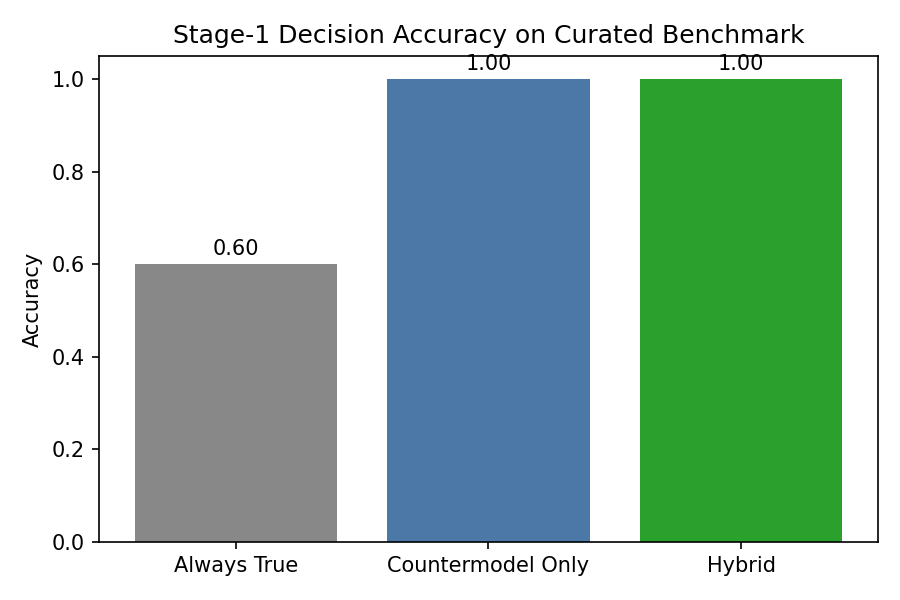
\includegraphics[width=0.78\linewidth]{figures/accuracy_comparison.png}
\caption{Accuracy comparison across baselines and the hybrid policy.}
\label{fig:acc}
\end{figure}

\begin{figure}[t]
\centering
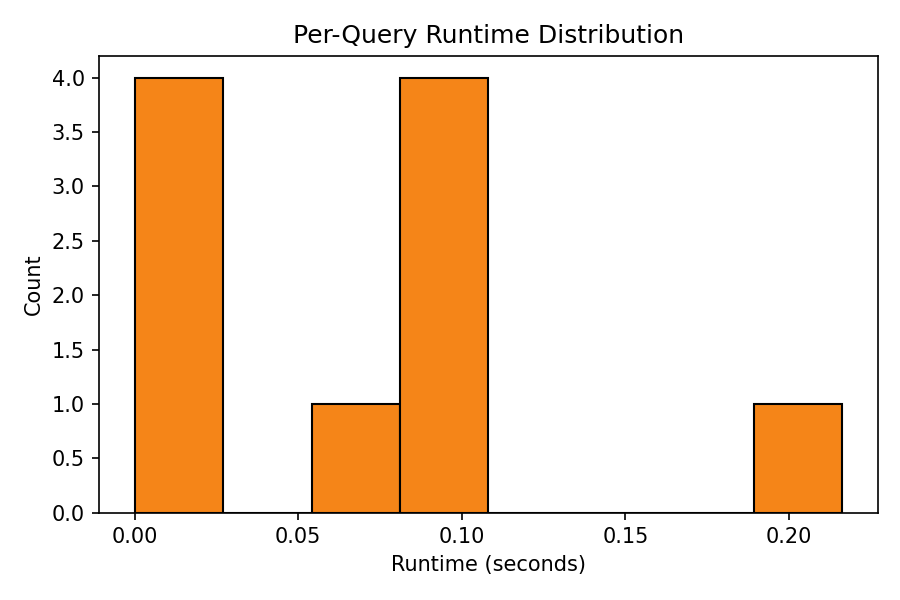
\includegraphics[width=0.78\linewidth]{figures/runtime_hist.png}
\caption{Runtime distribution over ten benchmark queries (mean $0.0623$ seconds).}
\label{fig:runtime}
\end{figure}

\begin{corollary}\label{cor:pilot}
On the curated benchmark, the solver is empirically correct and low-latency while preserving strict Stage-1 output format.
\end{corollary}

\begin{proof}
Combine Propositions~\ref{prop:boolean} and~\ref{prop:bench-correct} with the runtime statistics in \texttt{results/metrics.json}, and note from Theorem~\ref{thm:sound-negative} that every returned \texttt{false} is semantically justified by an explicit witness.
\end{proof}
